\RussianSourceFrame{GELFAND-P001455}{49}
% Original scan inspected directly. Reproducible review coordinates are retained in completion.json.
% Diagram (10): [100,50,645,435], 3x. Visible contour gaps and two unattached inner strokes retained.
\begin{center}
\begin{tikzpicture}[x=0.012cm,y=-0.012cm,line width=0.5pt]
\node at (145,215) {(10)};
\draw (255,217)--(256,160)--(310,87);
\draw (345,78)--(425,72)--(510,107)--(555,160)--(550,216)--(527,270);
\draw (507,303)--(402,321);
\draw (315,278)--(280,269)--(256,231);
\draw (360,155)--(410,200);
\draw (402,250)--(472,210);
\draw (550,216)..controls (620,196) and (652,394)..(539,429)..controls (480,426) and (433,376)..(402,321);
\draw (550,216) circle (6);
\draw (402,321) circle (6);
\node at (600,186) {$1$};
\node at (390,384) {$3$};
\end{tikzpicture}
\end{center}
Рассм. более сложную конфигурацию
и все возможные раскраски контур.
(в 4 цвета)

Нек-рые из них продолжаются внутрь,
а нек-рые нет.

Можно пробовать перекраски как в (9) (с пол. успех).
Этим способом компьютер ищет приводимые конфигурации.

% Diagram (11): [350,660,810,1085], 4x. Nodes, unarrowed edges and embedding directly checked.
\begin{center}
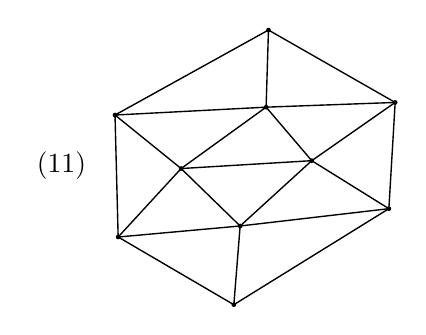
\begin{tikzpicture}[x=0.01cm,y=-0.01cm,line width=0.5pt]
\node at (335,870) {(11)};
\coordinate (a) at (598,698);
\coordinate (b) at (759,790);
\coordinate (c) at (751,925);
\coordinate (d) at (554,1047);
\coordinate (e) at (407,961);
\coordinate (f) at (403,806);
\coordinate (g) at (595,796);
\coordinate (h) at (487,874);
\coordinate (i) at (653,864);
\coordinate (j) at (562,947);
\draw (a)--(b)--(c)--(d)--(e)--(f)--(a);
\draw (a)--(g)--(b);
\draw (f)--(g)--(h)--(f);
\draw (h)--(e);
\draw (g)--(i)--(b);
\draw (h)--(i)--(c);
\draw (h)--(j)--(i);
\draw (e)--(j)--(c);
\draw (j)--(d);
\fill (a) circle (3);
\fill (b) circle (3);
\fill (c) circle (3);
\fill (d) circle (3);
\fill (e) circle (3);
\fill (f) circle (3);
\fill (g) circle (3);
\fill (h) circle (3);
\fill (i) circle (3);
\fill (j) circle (3);
\end{tikzpicture}
\end{center}
Приводимая конфигурация
(но Фуксу [зачёркнуто: \RussianUnclear{GELFAND-P001455}{configuration-cancel}{у / д}] не удалось доказать)

И.М.Г. \underline{Задача} \RussianUnclear{GELFAND-P001455}{task-number}{6 / в}.
Написать программу опред. приводимости для
параллельного компьютера.

Одна из конфигур. Аппеля и Хакена (из 1700) была проверена
вручную (Allaire), т.к. не бралась машиной.

\underline{Неизбежное мн-во.}

Их построение основано на теор. Эйлера
\begin{equation*}
\mathrm{В}-\mathrm{Р}+\mathrm{Г}=2.\tag{12}
\end{equation*}
\underline{Кемпе:} пусть \RussianUnclear{GELFAND-P001455}{vertex-count-symbol}{$\nu_i$ / $v_i$} — число вершин, к-рые соед. ровно
с $i$ другими вершинами (из них вых. $i$ рёбер)
\begin{equation*}
\mathrm{В}=\nu_3+\nu_4+\nu_5+\ldots\tag{13}
\end{equation*}
\begin{equation*}
\mathrm{Р}=\frac{1}{2}(3\nu_3+4\nu_4+5\nu_5+\ldots)\tag{14}
\end{equation*}
% Small incident-pair sketch: original approximately [280,2500,440,2610], reviewed in equations-middle at 3x.
\begin{center}
\begin{tikzpicture}[x=0.01cm,y=-0.01cm,line width=0.5pt]
\draw (298,2590) circle (5);
\draw (302,2585)--(430,2520);
\end{tikzpicture}
\end{center}
\begin{equation*}
2\mathrm{Р}=\text{число таких пар}=3\nu_3+4\nu_4+\ldots
\end{equation*}
(вершина и исх. из нее ребро)
\begin{equation*}
3\mathrm{Г}=2\mathrm{Р}\qquad\text{(т.к. триангуляция)}\tag{15}
\end{equation*}
отсюда
\begin{equation*}
\mathrm{Г}=\frac{3\nu_3+4\nu_4+5\nu_5+\ldots}{3}\tag{15'}
\end{equation*}
Из (12) находим:
\begin{equation*}
3\nu_3+2\nu_4+\nu_5-\nu_7-2\nu_8-3\nu_9-\ldots=12,\tag{16}
\end{equation*}
т.е.

[Зачёркнут номер: \RussianUnclear{GELFAND-P001455}{cancelled-equation-number}{(17) / (16)}]
\begin{equation*}
\sum_{i=3}^{\infty}(6-i)\nu_i=12\tag{16'}
\end{equation*}


\par\smallskip\noindent\leavevmode\phantomsection\label{GELFAND-P001455:recolouring-success-abbreviation:editorial}{\footnotesize\textbf{Редакторское сопоставление.} В источнике написано «с пол. успех.». Сокращение «пол.» проверено при 3×, 5× и 10×. Раскрытие до «полным» или «половинным» не установлено; буквальное сокращение сохранено.\par}\smallskip


\RussianSourceFrame{GELFAND-P001456}{unlabelled}
% Original scan inspected directly. Reproducible review coordinates are retained in completion.json.
(17) Отсюда одно из чисел \RussianUnclear{GELFAND-P001456}{vertex-count-symbol}{$\nu_3,\nu_4,\nu_5$ / $v_3,v_4,v_5$} отлично от $0$.

Получаем неизбежное мн-во

% Figure (18), first two sketches: [80,300,1680,710], 3x. The second crossing is not supplied with an invented central dot.
\begin{center}
\begin{tikzpicture}[x=0.018cm,y=-0.018cm,line width=0.5pt]
\node at (300,390) {(18)};
\draw (377,433)--(432,328)--(484,421)--(377,433);
\draw (377,433)--(430,391)--(484,421);
\draw[line width=1pt] (432,328)--(430,391);
\fill (430,391) circle (3);
\draw (405,490)--(405,550);
\node at (435,590) {привод.};
\draw (609,372)--(667,325)--(761,355)--(657,434)--(609,372);
\draw (609,372)--(761,355);
\draw (667,325)--(657,434);
\draw (685,490)--(685,550);
\node at (685,590) {привод.};
\end{tikzpicture}
\end{center}
\RussianSourceFigure{GELFAND-P001456}{diagram-18-right}{Третий рисунок в (18): пятиугольный контур с верхней вершиной, двумя боковыми и двумя нижними вершинами; внутри отмечен узел, от которого проведены пять отрезков к вершинам контура. Верхняя правая сторона обведена густым клиновидным штрихом; у её правого конца есть короткий выступ, характер которого неясен. Под рисунком вертикальный указатель к надписи «не удаётся сразу / док. приводимость».}

\par\medskip\noindent
\begin{minipage}[c]{0.48\linewidth}\centering
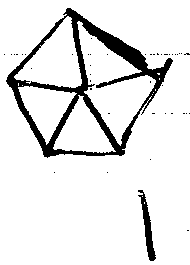
\includegraphics[width=\linewidth]{figures/gelfand-p001456-diagram-18-right-original-r2.png}
\par\smallskip{\footnotesize Оригинал рукописного рисунка: GELFAND-P001456\par}
\end{minipage}\hfill
\begin{minipage}[c]{0.48\linewidth}\centering
\resizebox{\linewidth}{!}{% Visible strokes only: the thick wedge is not asserted to be an arrow.
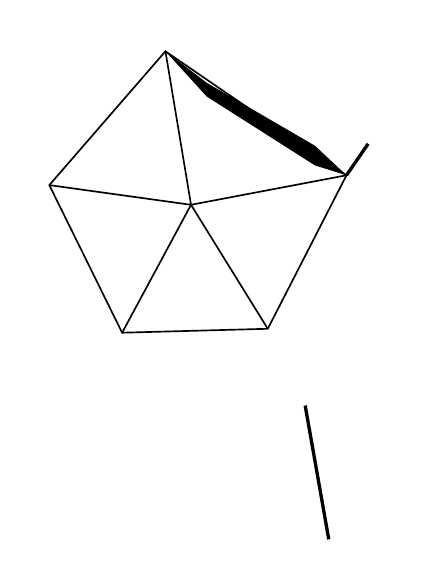
\begin{tikzpicture}[x=0.025cm,y=-0.025cm,line width=0.6pt]
\path[use as bounding box] (0,0) rectangle (190,265);
\draw (11,80)--(70,12)--(162,75)--(122,153)--(48,155)--cycle;
\draw (70,12)--(83,90)--(11,80);
\draw (48,155)--(83,90)--(122,153);
\draw (83,90)--(162,75);
\fill (70,12)--(91,28)--(146,60)--(162,75)--(146,70)--(91,35)--cycle;
\draw[line width=1.2pt] (162,75)--(173,59);
\draw[line width=1.2pt] (141,192)--(153,260);
\end{tikzpicture}
}
\par\smallskip{\footnotesize Частичное воссоздание видимых штрихов; неясные соединения и подписи отмечены.\par}
\end{minipage}\par\medskip


Теперь можно рассм. лишь триангул. с
\begin{equation*}
\nu_3=\nu_4=0\tag{19}
\end{equation*}
\underline{Discharging} (разрядка)

(20) Начальный заряд: вершине, из к-рой исх. $i$ рёбер,
припиш. заряд [зачёркнуто: \RussianUnclear{GELFAND-P001456}{initial-charge-cancel}{$60-i$ / $6-i$}] $60(6-i)$

\underline{Процедура перезарядки:} строим другую ф-ю на вершинах.
\begin{equation*}
(16')\Longleftrightarrow\text{сумма всех зарядов}=720.
\end{equation*}
(21) Хотим [надстрочная вставка: «сделать»], чтобы все заряды были $\leq0$.

(что невозможно [зачёркнуто: \RussianUnclear{GELFAND-P001456}{impossible-cancel}{неразборчиво}] ввиду равенства (16'))

\underline{1 процедура.}

% Figure (22): line without an arrowhead, open left endpoint and dark right endpoint; [65,1565,2210,2150], 3x.
\begin{center}
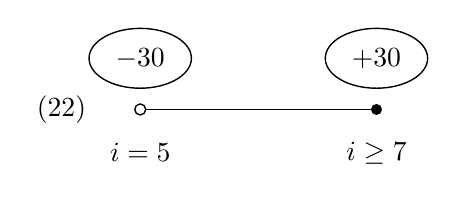
\begin{tikzpicture}[line width=0.5pt]
\node at (-1,0) {(22)};
\draw (0.07,0)--(3,0);
\draw (0,0) circle (0.07);
\fill (3,0) circle (0.07);
\draw (0,0.65) ellipse (0.65 and 0.38);
\node at (0,0.65) {$-30$};
\draw (3,0.65) ellipse (0.65 and 0.38);
\node at (3,0.65) {$+30$};
\node at (0,-0.55) {$i=5$};
\node at (3,-0.55) {$i\geq7$};
\end{tikzpicture}
\end{center}
(в 1-й вершине уменьшаем на 30,
во 2-й — увелич. на 30)

\underline{Неск. ситуаций, когда остается полож. заряд где-то}

(23) $1^{\circ}$.
\begin{tikzpicture}[baseline=0pt]
\draw (0,0) circle (0.055);
\node at (0.3,0.45) {5 рёбер};
\end{tikzpicture}
соед. с $0$ или $1$ [зачёркнуто: \RussianUnclear{GELFAND-P001456}{situation-one-cancel}{рёбр / рёбер}] верш. с числом рёбер $\geq7$

($\Rightarrow$ ост. вершина с полож. зарядом

[Отдельно зачёркнут знак: \RussianUnclear{GELFAND-P001456}{cancelled-enumeration}{2 / неразборчиво}]

(24) $2^{\circ}$.
\begin{tikzpicture}[baseline=0pt]
\fill (0,0) circle (0.055);
\node at (0,-0.5) {кр. 7};
\end{tikzpicture}
соед. [зачёркнуто: \RussianUnclear{GELFAND-P001456}{situation-two-cancel}{ребра с / ребро с}] с $\leq2$ вершин кратности $5$

В итоге получ. конечный набор конфигур., к-рый неизбежен,
т.к. если нет ни одной из них, то можно сделать все
заряды $\leq0$.


\par\smallskip\noindent\leavevmode\phantomsection\label{GELFAND-P001456:case24-charge-inequality:editorial}{\footnotesize\textbf{Редакторское сопоставление.} В случае (24) написано $\le2$, что подтверждено при 3×, 5× и 10×. При указанной передаче 30 от каждой смежной вершины кратности 5 заряд вершины кратности 7 равен $-60+30k$ и неположителен при $k\le2$. Этот локальный расчёт не даёт положительного заряда у данной вершины, но не опровергает более широкого утверждения о положительном заряде где-то и не даёт основания заменять знак на $\ge3$.\par}\smallskip


\RussianSourceFrame{GELFAND-P001457}{50}
% Original scan inspected directly. Reproducible review coordinates are retained in completion.json.
Теперь надо проверить их на приводимость.

Авторы (Аппель и Хакен) в 1977 г. благодарят администр.
за 12000 часов маш. времени.
[Число 12000 волнисто подчёркнуто; под ним: «(1200?)».]

Дальше конфигур. перестраиваются в более сложные и
правила переноса тоже.

\underline{\underline{А. Бейлинсон}} (продолжение)

(о раб. К. Вилонен, С. Гельфанд, Р. Д. Макферсон)

[Под «Д.» указателем приписано: «Дункан».]

$X$ — гладкое [надстрочная вставка: «комплексное»] алгебр. мн-зие,

$\mathcal{F}$ — конечномерный констр. [зачёркнуто: «пучок»; надстрочная замена: «комплекс пучков»] на $X$.

По этим данным строится

$\mathrm{SS}(\mathcal{F})$ — лагранжево коническое мн-зие в
[зачёркнуто: $T^*X$] $\Omega X=T^*X$.

$\mathrm{SS}(\mathcal{F})=\text{нулевое сеч.}\Longleftrightarrow H^i(\mathcal{F})$ гладкий, т.е. локально постоянен

\underline{Опр.} $\mathrm{SS}\mathcal{F}$

\begin{equation*}
H^\bullet(\mathcal{F})=0\quad\Rightarrow\quad\mathrm{SS}(\mathcal{F})=\varnothing\tag{1}
\end{equation*}
\begin{equation*}
H^\bullet(\mathcal{F})\neq0\quad\Rightarrow\quad\mathrm{SS}(\mathcal{F})\supset\text{нулевое сечение},\quad\text{а}
\end{equation*}
$\mathrm{SS}(\mathcal{F})\setminus(\text{нулевое сечение})$ опис. следующим образом
\begin{equation*}
\nu\in\Omega_x^1,\qquad\text{выберем }f:\quad df_x=\nu,\quad f(x)=0
\end{equation*}
[Под $\nu$ указателем приписано: «вектор».]

Пусть $U$ — маленькая окр. точки $x$
\begin{equation*}
H^\bullet(U,U\cap f^{-1}(\varepsilon)\text{[зачёркнуто: }\mathcal{F}\text{]};\mathcal{F})
=\Phi_f^\bullet(\mathcal{F})_x\tag{2}
\end{equation*}
(пр-во исчезающих [зачёркнуто: \RussianUnclear{GELFAND-P001457}{vanishing-cycles-cancel}{коциклов / когомол.}] циклов)

$\varepsilon\neq0$ мало

(\RussianUnclear{GELFAND-P001457}{hypercohomology-word}{гипергомологии / гиперкогомологии})

(относит. когом. опред. через конус)
отобр., т.е. надо напис. бикомплекс и
свернуть

% Commutative square: [240,2855,2350,3410], 3x. Both upper exponents read as 1 after 10x reviews [425,3010,515,3130] and [850,3000,950,3110].
\begin{equation*}
\begin{tikzcd}
\mathcal{F}^1(U) \arrow[r] & \mathcal{F}^1(U\cap f^{-1}(\varepsilon)) \\
\mathcal{F}^0(U) \arrow[r] \arrow[u] & \mathcal{F}^0(U\cap f^{-1}(\varepsilon)) \arrow[u]
\end{tikzcd}
\end{equation*}
(если $\mathcal{F}$ достаточно
ацикличен)


\RussianSourceFrame{GELFAND-P001458}{unlabelled}
% Original scan inspected directly. Reproducible review coordinates are retained in completion.json.
объяснение того, [зачёркнуто: \RussianUnclear{GELFAND-P001458}{top-cancellation}{почему / зачем}; над строкой вставлено: при чём] здесь исчезающие циклы.

\RussianSourceFigure{GELFAND-P001458}{vanishing-cycle-sketch}{Вверху слева несколько дуг сходятся в одну точку; справа узкий заштрихованный овал между двумя дугами. Ниже горизонтальный овал с двумя точками и соединяющим их штрихом с головкой у левой точки. От верхнего правого овала к правой нижней точке идёт прерывистая линия. Точная геометрия и направление отдельных штрихов требуют сверки с оригиналом.}

\par\medskip\noindent
\begin{minipage}[c]{0.48\linewidth}\centering
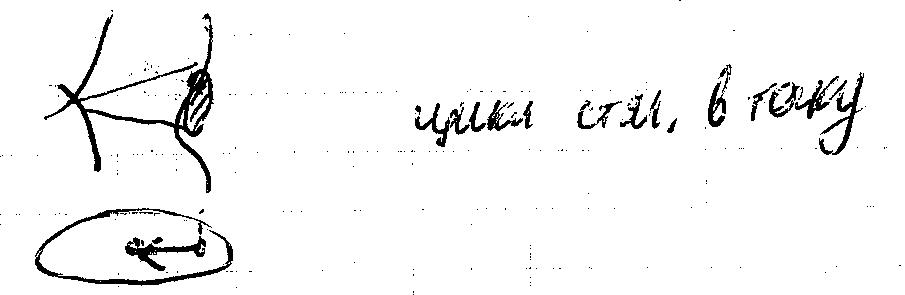
\includegraphics[width=\linewidth]{figures/gelfand-p001458-vanishing-cycle-sketch-original.png}
\par\smallskip{\footnotesize Оригинал рукописного рисунка: GELFAND-P001458\par}
\end{minipage}\hfill
\begin{minipage}[c]{0.48\linewidth}\centering
\resizebox{\linewidth}{!}{\def\VanishingCycleCaption{цикл стя[н/г]. в точку}
% Partial trace: hatching, lower left head and broken vertical strokes retained.
\begin{tikzpicture}[x=0.01cm,y=-0.01cm,line width=0.55pt]
\path[use as bounding box] (0,0) rectangle (905,295);
\draw (45,86)--(75,102)--(45,118);
\draw (75,102)..controls(92,76)and(103,35)..(112,13);
\draw (75,102)..controls(88,124)and(95,149)..(98,170);
\draw (75,102)--(200,65);
\draw (75,102)..controls(111,122)and(149,125)..(185,130);
\draw (207,15)..controls(218,35)and(205,65)..(200,65);
\draw (200,65)..controls(217,84)and(215,117)..(191,136)
 ..controls(170,135)and(176,109)..(188,84)..controls(195,76)and(198,70)..(200,65);
\draw (191,136)..controls(205,151)and(212,173)..(208,190);
\draw (189,89)--(204,74);\draw (182,107)--(208,79);
\draw (179,123)--(209,92);\draw (184,132)--(204,108);
\draw (132,249) ellipse [x radius=99,y radius=37];
\fill (140,250) circle[radius=2];\fill (199,249) circle[radius=2];
\draw (140,250)--(199,249);\draw (154,242)--(140,250)--(160,268);
\draw (200,210)--(200,217);\draw (199,225)--(199,233);\draw (199,240)--(199,245);
\node[anchor=west,text width=4.5cm,align=left] at (400,110) {\VanishingCycleCaption};
\end{tikzpicture}
}
\par\smallskip{\footnotesize Частичное воссоздание видимых штрихов; неясные соединения и подписи отмечены.\par}
\end{minipage}\par\medskip


[Справа от рисунка:] цикл \RussianUnclear{GELFAND-P001458}{cycle-caption}{стян. / стяг.} в точку

\underline{Df.} $\nu\notin SS(\mathcal F)\Longleftrightarrow$ исчез. циклы в $\nu$ равны $0$, т.е. \RussianUnclear{GELFAND-P001458}{vanishing-cycles-degree}{$\Phi_f^i(\mathcal F)_x=0$ / $\Phi_f^\bullet(\mathcal F)_x=0$ / $\Phi_f^*(\mathcal F)_x=0$}.

Рассм. прямой образ $\mathcal F|_U$ при отобр. $U\overset{f}{\longrightarrow}\text{диск}$.

Исчез. циклы меряют, насколько слой в т. $0$ отличается от соседних слоёв.

$f$ наз. \underline{морсовской} ф-ей на $X$, если [над строкой вставлено: $f$ голоморфная ф-я на $X$ и] график $df(X)\subset$ [зачёркнуто: \RussianUnclear{GELFAND-P001458}{cotangent-cancellation}{неразборчивый знак}] $\Omega^1$ трансверсально пересекает $SS(\mathcal F)$.

Комплекс наз. \underline{извращ. пучком}, если $\forall$ морсовской отн. $\mathcal F$ ф-и имеются исчез. циклы лишь в размерности $0$.

(только $\Phi_f^0(\mathcal F)\neq0$)

$\mathcal F$ — извращ. пучок.

По нему строится \underline{лок. система на рег. точках син. носителя}.

Её слой над точкой $\nu$:
\begin{equation*}
\Phi(\mathcal F)_\nu=\Phi_f^0(\mathcal F)_x
\end{equation*}
для морсовской ф-и $f$ с $df(x)=\nu$, \RussianUnclear{GELFAND-P001458}{normalization-argument}{$f(0)=0$}.

Что происходит в особых точках?

\underline{Задача}: описать извр. пучки микролокальным способом,
т.е. в терминах исчез. циклов.

Она решена в работе наполовину.

\underline{Смысл}: откуда берутся извращ. пучки?

$1^\circ$. $\mathcal M$ — переопр. система

[Под словом «система»:] (голон.)

[Справа:] $\sum f_i\partial^i$

[Под $f_i$ вертикальная черта к подписи:] голом.

\begin{equation*}
\mathcal F^{0,0}\overset{\bar\partial}{\longrightarrow}\mathcal F^{0,1}\longrightarrow\cdots
\end{equation*}

[Над началом следующей строки отдельный знак:] \RussianUnclear{GELFAND-P001458}{lower-detached-mark}{4 / знак вставки}

если $u\in\mathcal F^{0,0}$ — решение $\mathcal M$, то $\bar\partial u$ тоже

Система переопред, $\Rightarrow$ комплекс решений — извращ. пучок.


\RussianSourceFrame{GELFAND-P001459}{51}
% Original scan inspected directly. Reproducible review coordinates are retained in completion.json.
$2^\circ$. Комбинаторный способ

(Горески — Макферсон)

Есть [вставлено над строкой: общий] способ продолжения пучков в особ. точки $\Rightarrow$ получаются [зачёркнуто: \RussianUnclear{GELFAND-P001459}{upper-cancellation}{неразборчивое слово}] извращ. пучки.

Работа посвящена $3$-му способу.

\underline{След. раз} $(18/\mathrm{IV})$ докл. \underline{Решетихина} о квант. группах.

[Ниже горизонтальная черта. Под ней у нижнего края текстового фрагмента: \RussianUnclear{GELFAND-P001459}{bottom-cutoff}{обрезанные штрихи, возможно «М...»}.]


\RussianSourceFrame{GELFAND-P001460}{unlabelled}
% Original scan inspected directly. Reproducible review coordinates are retained in completion.json.
\underline{18.4.1988 г.}\qquad \underline{\underline{Сем. Гельфанда.}}

% The following heading has a wavy underline in the source. The author names in the left margin have broken underlines.
\underline{Назв. докладов сем. Бурбаки} $(87-88\text{ г.})$

\underline{Лернер.}\quad "Принцип неопр. и микролокализация" (по Феферману и Фонгу)

"Геом. полиномов и метод Ньютона" (по Смейлу и Шубу)

"Смешанные нелин. задачи"

"Некоммут. стох. исчисление"

"Метаплектич. предст. и гипотеза Хау"

"Пробл. Шоттки и гип. Новикова"

\underline{Дуади.}\quad "Диски Зигеля и кольцо Хермана"

"Деформации плоских кривых"

"Большие уклонения"

"Классиф. унитарных предст. вещ. групп"

"Теория классификации"

"Стаб. пучки и [зачёркнуто: \RussianUnclear{GELFAND-P001460}{stable-cancellation}{неразборчивое слово}]
% No clear closing quotation mark survives after the cancelled material.

"Moonshine"

\underline{Вердье.}\quad "Квант. группы\RussianUnclear{GELFAND-P001460}{quantum-title-mark}{[надстрочный знак: зачёркнутые кавычки / звёздочка]} (по Дринфельду)"

\underline{Мальгранж.}\quad "Геометрич. преобр. Фурье"

"Новые инварианты гомологич. сфер разм. $3$"

"Эллиптич. когомологии"

"Посл. достижения в теор. Ферма".


\RussianSourceFrame{GELFAND-P001461}{63}
% Original scan inspected directly. Reproducible review coordinates are retained in completion.json.
% Source has a straight underline under the surname and a wavy underline under «о раб. Атьи».
\underline{Бейлинсон} \underline{о раб. Атьи} и кого-то ещё.

\underline{Полубесконечная теория Морса.}

В $\infty$-мерном случае есть 2 вар. теории Морса (для вычисл. гомологий).

1) Зад. о геодезич. с ф-лом энергии похожа на конечномерную.
Отриц. индекс инерции конечен и равен числу сопр. точек на геодезической.

2) $\infty$-мерн. мн-зие, ф-л типа энергии
с изолир. критич. точками, но с $\infty$ числом $+$ и $\infty$ числом $-$.
Но оказ., что у двух разных крит. точек число $-$ отлич. на конечное
число; строятся гомологии, отсчит. от $\infty/2$
(топ. вариант Фейгина и Цыгана)

% «Сенсация» is wavy-underlined in the source.
\underline{Сенсация}: эти инвар. связаны с инвариантами Дональдсона
4-мерных мн-зий.

% Diagram at source (250,1285,910,1515): vertical oval, wider partly dashed outline, right arrow to M.
\begin{center}
\begin{tikzpicture}[x=1cm,y=1cm]
\draw (0,0) ellipse (0.30 and 0.43);
\draw (-0.30,0.44) .. controls (-0.18,0.47) and (-0.08,0.44) .. (0.01,0.44);
\draw (0.02,0.49) .. controls (0.39,0.66) and (0.67,0.30) .. (0.48,-0.04);
\draw (-0.76,0.17) .. controls (-0.88,0.11) and (-0.85,0.00) .. (-0.84,-0.11);
\draw (-0.82,-0.33) .. controls (-0.72,-0.39) and (-0.62,-0.43) .. (-0.55,-0.45);
\draw (-0.34,-0.51) .. controls (-0.20,-0.50) and (-0.13,-0.58) .. (-0.04,-0.53);
\draw (0.19,-0.46) -- (0.39,-0.35);
\draw[->] (0.98,0.02) -- (2.38,0.02);
\node at (2.84,0.02) {$M$};
\node at (0.40,-0.91) {$S^1\subset\mathbb C P^1$};
\node at (2.93,-0.91) {(напр. $\mathbb C$)};
\end{tikzpicture}
\end{center}

Выделим для $S^1\to\mathbb C$ 2 половинки (продолж. внутрь и наружу);
они пересек. по конечномерному мн-зию.

\RussianSourceFigure{GELFAND-P001461}{surface-sketch}{Слева овальный контур с двумя маленькими петлеобразными штрихами внутри; снаружи более широкий, частично пунктирный контур. Точное соединение верхнего внутреннего штриха с контуром и смысл внутренних петель требуют сверки с оригиналом.}

\par\medskip\noindent
\begin{minipage}[c]{0.48\linewidth}\centering
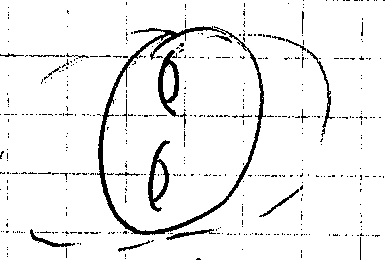
\includegraphics[width=\linewidth]{figures/gelfand-p001461-surface-sketch-original-r2.png}
\par\smallskip{\footnotesize Оригинал рукописного рисунка: GELFAND-P001461\par}
\end{minipage}\hfill
\begin{minipage}[c]{0.48\linewidth}\centering
\resizebox{\linewidth}{!}{% Partial stroke trace; no genus, handle attachment or missing join is inferred.
\begin{tikzpicture}[x=0.02cm,y=-0.02cm,line width=0.55pt]
\path[use as bounding box] (0,0) rectangle (385,260);
\draw (190,30)..controls(145,34)and(112,95)..(100,155)
 ..controls(92,196)and(100,220)..(130,230)
 ..controls(165,242)and(220,205)..(241,158)
 ..controls(269,103)and(268,59)..(235,40)..controls(221,27)and(204,28)..(190,30);
\draw (174,53)..controls(156,67)and(153,85)..(160,103)
 ..controls(168,118)and(179,103)..(177,78)..controls(174,67)and(169,61)..(168,61);
\draw (160,103)..controls(164,110)and(169,113)..(176,116);
\draw (169,141)..controls(155,143)and(149,169)..(150,193)
 ..controls(151,207)and(159,214)..(163,207);
\draw (159,159)..controls(177,174)and(171,187)..(151,201);
\draw (131,34)..controls(144,28)and(164,28)..(178,32);
\draw (240,35)..controls(288,35)and(329,47)..(329,92);
\draw (329,94)..controls(334,112)and(326,130)..(323,143);
\draw (300,186)--(273,207)--(260,214);
\draw (250,231)--(200,240);\draw (155,237)--(120,247);
\draw (94,242)--(68,244)--(32,235);\draw (42,81)--(63,66);
\end{tikzpicture}
}
\par\smallskip{\footnotesize Частичное воссоздание видимых штрихов; неясные соединения и подписи отмечены.\par}
\end{minipage}\par\medskip

[Под рисунком:] рим. пов. $\subset$ сфера

[Справа от рисунка:] калибр. поля; ф-л Я.-М.
крит. точки — плоские связности.

\underline{И.М.Г.} Разлож. $C^\infty(S^1)$ эксплуатировалось нами ($\sim20$ лет)
(в т.ч. $\tau$-ф-и Хирота-Сато, $\frac12$-когомологии)

Замечательно, что можно заменить $S^1$ другими мн-зиями.
Это будет в след. раз.

\underline{\underline{Решетихин}} \underline{Коля}.

[Зачёркнуто и подчёркнуто: Квантовые группы.]

$\underline{U_q(SU(2))}$ \underline{и инварианты зацеплений и предст. группы кос.}

\begin{equation*}
A=\underset{\text{ассоц. алг.}}{U_q(SU(2))};\qquad
1,H,X^\pm\quad\text{— образующие}
\end{equation*}
\begin{equation*}
[X^\pm,H]=\mp2X^\pm;
\tag{1}
\end{equation*}
\begin{equation*}
[X^+,X^-]=\frac{\operatorname{sh}\left(\frac h2 H\right)}{\operatorname{sh}(h/2)};
\qquad q=e^h
\end{equation*}


\RussianSourceFrame{GELFAND-P001462}{unlabelled}
% Original scan inspected directly. Reproducible review coordinates are retained in completion.json.
% Basis monomial is wavy-underlined in source; denominator of the exponent is 4 (7x review).
\begin{equation*}
\underline{\left(q^{H/4}\right)^\ell H^n(X^+)^m(X^-)^k}
\quad\text{— базис как лин. пр-ва}
\tag{2}
\end{equation*}

\begin{equation*}
\Delta:A\to A\otimes A
\end{equation*}
\begin{equation*}
\Delta(H)=H\otimes1+1\otimes H
\tag{3}
\end{equation*}
\begin{equation*}
\Delta(X^\pm)=X^\pm\otimes q^{H/4}+q^{-H/4}\otimes X^\pm
\end{equation*}

1. $\Delta$ — гом. алгебр. $\Delta(ab)=\Delta(a)\Delta(b)$

2. $\Delta$ — коассоц., т.е.
\begin{center}
\begin{tikzcd}[column sep=large,row sep=large]
& A\otimes A \arrow[dr,"\mathrm{id}\otimes\Delta"] & \\
A \arrow[ur,"\Delta"] \arrow[dr,"\Delta"'] & & A\otimes A\otimes A \\
& A\otimes A \arrow[ur,"\Delta\otimes\mathrm{id}"'] &
\end{tikzcd}
\end{center}
[Справа:] (ал. Хопфа)

3. [Зачёркнуто: \RussianUnclear{GELFAND-P001462}{antipode-cancelled-sign}{неразборчивый знак}.]
$S:A\to A$ антигомоморфизм (аналог перех. к обр.
элементу в алгебре ф-й на группе)

\begin{equation*}
S(X^\pm)=q^{H/2}X^\pm q^{-H/2}
\tag{4}
\end{equation*}
\RussianUnclear{GELFAND-P001462}{antipode-formula}{[Формула (4): так в источнике.]}
\begin{equation*}
S(H)=-H
\end{equation*}
\begin{equation*}
\epsilon(H)=\epsilon(X^\pm)=0
\end{equation*}

\begin{center}
\begin{tikzcd}[column sep=large,row sep=large]
& A\otimes A \arrow[r,shift left=1.2ex,"S\otimes\mathrm{id}"] \arrow[r,shift right=1.2ex,"\mathrm{id}\otimes S"'] & A\otimes A \arrow[dr,"m"] & \\
A \arrow[ur,"\Delta"] \arrow[drr,"\epsilon"'] & & & A \\
& & \mathbb C \arrow[ur,"e"'] &
\end{tikzcd}
\end{center}
[Справа:] (можно брать любую из стрелок)

Превр. в квадр. алгебру в [Вставлено над строкой: других] образующих
[Зачёркнуто: \RussianUnclear{GELFAND-P001462}{cancelled-generators}{возможно, $K,X^\pm$, затем неразборчивые штрихи}.]

Рассм.
\begin{equation*}
K=q^{H/2},\qquad K,X^\pm
\end{equation*}
[Слева зачёркнуто: $K,X^\pm$.]
\begin{equation*}
KX^\pm=q^{\pm1}X^\pm K
\end{equation*}
\begin{equation*}
X^+X^- -X^-X^+=\frac{K-K^{-1}}{q-q^{-1}}
\end{equation*}
\RussianUnclear{GELFAND-P001462}{commutator-normalization}{[Знаменатель $q-q^{-1}$: так в источнике.]}


\RussianSourceFrame{GELFAND-P001463}{64}

(5) инволюция
\begin{equation*}
(X^+)^*=X^-,\qquad H^*=H
\end{equation*}

конечномерные предст.
\begin{equation*}
\pi_j(X^{\pm})e_m^j=
\sqrt{\frac{\operatorname{sh}\bigl(\frac h2(j\mp m)\bigr)
\operatorname{sh}\bigl(\frac h2(j\pm m+1)\bigr)}
{\operatorname{sh}^{2}\bigl(\frac h2\bigr)}}\,e_{m\pm1},
\qquad j\in\mathbb Z/2,
\qquad -j\le m\le j
\tag{6}
\end{equation*}
\begin{equation*}
\dim V^j=2j+1\quad\text{(как для $\mathrm{SL}_2$)}
\end{equation*}

Склянин писал в квадр. алгебрах.

\underline{Упражн.} \underline{(И. М. Г.)} $q=1\ \Rightarrow$ ф-лы из кн. Гельф.-Минлос-Шапиро

[Справа, выделено скобкой:] \underline{конкр. зад.}: как разл. вект. поля на сфере по сферич. \RussianUnclear{GELFAND-P001463}{exercise-harmonics}{гар-ям / гар-м}

начать с $\mathrm{SU}(2)$

(7) \underline{Теор.} Положим
\begin{equation*}
R=\exp\left(\frac h4 H\otimes H\right)
\sum_{n\ge0}\frac{q^n}{[n]_q!}\,e^n\otimes f^n
\tag{8}
\end{equation*}
\RussianUnclear{GELFAND-P001463}{r-coefficient}{Коэффициент в (8): $q^n/[n]_q!$ [так в записи].}
\begin{equation*}
R\in U_q(\mathrm{SU}(2))^{\otimes2},
\end{equation*}
где
\begin{equation*}
e=q^{H/4}X^+,\qquad f=q^{-H/4}X^-,
\tag{9}
\end{equation*}

(10) 1.
\begin{equation*}
(\Delta\otimes\mathrm{id})R=R_{23}R_{13},
\qquad (\in U_q(\mathrm{SU}(2))^{\otimes3})
\end{equation*}
[Перед скобкой справа зачёркнуто: \RussianUnclear{GELFAND-P001463}{cancelled-before-membership}{неразборчиво}.]
\begin{equation*}
(\mathrm{id}\otimes\Delta)R=R_{12}R_{13};
\end{equation*}
\begin{equation*}
2.\quad \sigma\circ\Delta(a)=R\,\Delta(a)R^{-1};\qquad\text{(см. (12))}
\end{equation*}
\begin{equation*}
3.\quad R_{12}R_{13}R_{23}=R_{23}R_{13}R_{12}.
\end{equation*}
[Справа:] (ур-е Янга-Бакстера со знач. в тенз. произв. 3-х экз. $A$)

В ф-ле (8)
\begin{equation*}
[n]_q!=[n]_q\ldots[1]_q\qquad\text{($q$-факториал)}
\tag{11}
\end{equation*}

\underline{И. М. Г.} Квантовая мех. — правильный способ вводить $q$.

\underline{\underline{Упр.}} что такое $\Gamma_q$?

\begin{equation*}
\sigma\colon A^{\otimes2}\longrightarrow A^{\otimes2},\qquad
\sigma(f\otimes g)=g\otimes f
\tag{12}
\end{equation*}
В частности, из $(10)_2$ следует, что $\sigma\circ\Delta$ — тоже коумножение.


\RussianSourceFrame{GELFAND-P001464}{unlabelled}

Определим
\begin{equation*}
R^{j_1j_2}\colon V^{j_1}\otimes V^{j_2}\longrightarrow V^{j_2}\otimes V^{j_1}
\end{equation*}
\RussianUnclear{GELFAND-P001464}{definition-separator}{После $R^{j_1j_2}$ исправленный знак: $:$; первоначальные штрихи неразборчивы.}

$V^j$ — пр-во конечномерн. предст.

\begin{equation*}
R^{j_1j_2}=P^{j_1j_2}\,\pi^{j_1}\otimes\pi^{j_2}(R)
\tag{13}
\end{equation*}
[Под $P^{j_1j_2}$, соединено чертой:] опер. перестановки пр-в

\begin{equation*}
\begin{aligned}
&(1\otimes R^{j_1j_2})(R^{j_1j_3}\otimes1)(1\otimes R^{j_2j_3})=\\
&\qquad=(R^{j_2j_3}\otimes1)(1\otimes R^{j_1j_3})(R^{j_1j_2}\otimes1)
\end{aligned}
\tag{14}
\end{equation*}

$q$-аналоги [зачёркнуто: \RussianUnclear{GELFAND-P001464}{cancelled-coefficient}{неразборчивый знак}] коэфф. Клебша-Гордана.

все конечномерн. предст. вполне прив.

\begin{equation*}
V^{j_1}\otimes V^{j_2}=\sum_{|j_1-j_2|\le j_3\le j_1+j_2}^{\oplus}V^{j_3}
\tag{15}
\end{equation*}
\RussianUnclear{GELFAND-P001464}{sum-mark}{Знак над суммой: $\oplus$; возможно, исправление $\otimes$ на $\oplus$.}

$V_j$ нашли Кулиш и Решетихин (1981)

В базисе:
\begin{equation*}
e_{m_1}^{j_1}\otimes e_{m_2}^{j_2}=
\sum_{|j_1-j_2|\le j_3\le j_1+j_2}
\begin{bmatrix}
j_1&j_2&j_3\\
m_1&m_2&m_3
\end{bmatrix}e_{m_3}^{j_3}
\tag{16}
\end{equation*}
[От квадратной скобки проведена черта к подписи:] коэфф. Клебша-Гордана

где
\begin{equation*}
m_3=m_1+m_2
\end{equation*}

Графич. запись:
\begin{equation*}
A\colon V^{j_1}\otimes\ldots\otimes V^{j_N}
\longrightarrow V^{j'_1}\otimes\ldots\otimes V^{j'_L}
\end{equation*}

(17)
\begin{center}
\begin{tikzpicture}[x=1cm,y=1cm]
\draw (0,0.08)--(0,1.65)--(3.25,1.65)--(3.25,0)--(0,0);
\node at (1.63,0.82) {$A$};
\draw (0.35,1.65)--(0.35,2.55);
\draw (1.25,1.65)--(1.25,2.55);
\draw (3.1,1.65)--(3.1,2.55);
\node[left] at (0.25,2.28) {$j'_1$};
\node[left] at (1.15,2.28) {$j'_2$};
\node at (2.2,2.15) {$\ldots$};
\node[right] at (3.1,2.28) {$j'_L$};
\draw (0.4,0)--(0.4,-1);
\draw (1.35,0)--(1.35,-1);
\draw (2.97,0)--(2.97,-0.87);
\node[below] at (0.13,-1.04) {$j_1$};
\node[below] at (1.17,-1.04) {$j_2$};
\node[below] at (3.15,-1.04) {$j_N$};
\end{tikzpicture}
\end{center}

\begin{equation*}
A^{m'_1\ldots m'_N}_{m_1\ldots m_L}
\end{equation*}
\RussianUnclear{GELFAND-P001464}{coefficient-range}{Индексы коэффициента: сверху $m'_1\ldots m'_N$, снизу $m_1\ldots m_L$ [так в записи].}
\begin{equation*}
-j_i\le m_i\le j_i;
\end{equation*}

[Справа внизу:]
\RussianSourceFigure{GELFAND-P001464}{diagram-02}{Прямоугольник с $A$ и тремя вертикальными выводами сверху и снизу, без стрелок. У верхних выводов: $j'_1$, $j'_2$, $j'_L$; над ними: $m'_1$, $m'_2$, многоточие, $m'$ с исправленным последним индексом ($L$ или $N$). У нижних выводов: $j_1$, $j_2$, $j_N$; ниже: $m_1$, $m_2$, $m_N$. Требует проверки исходный знак под исправленным верхним правым индексом.}

\par\medskip\noindent
\begin{minipage}[c]{0.48\linewidth}\centering
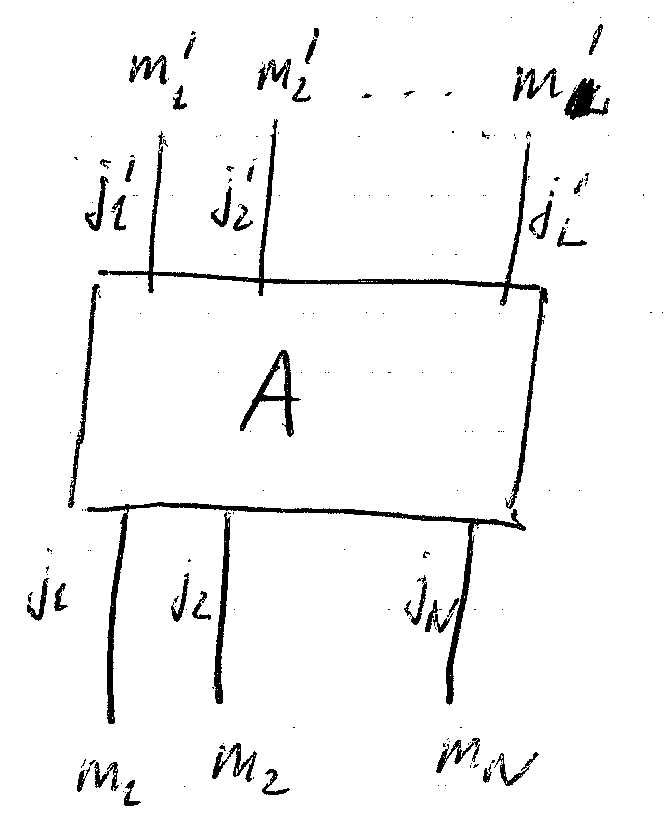
\includegraphics[width=\linewidth]{figures/gelfand-p001464-diagram-02-original.png}
\par\smallskip{\footnotesize Оригинал рукописного рисунка: GELFAND-P001464\par}
\end{minipage}\hfill
\begin{minipage}[c]{0.48\linewidth}\centering
\resizebox{\linewidth}{!}{% All clear source labels are typed. The overwritten last upper index stays uncertain.
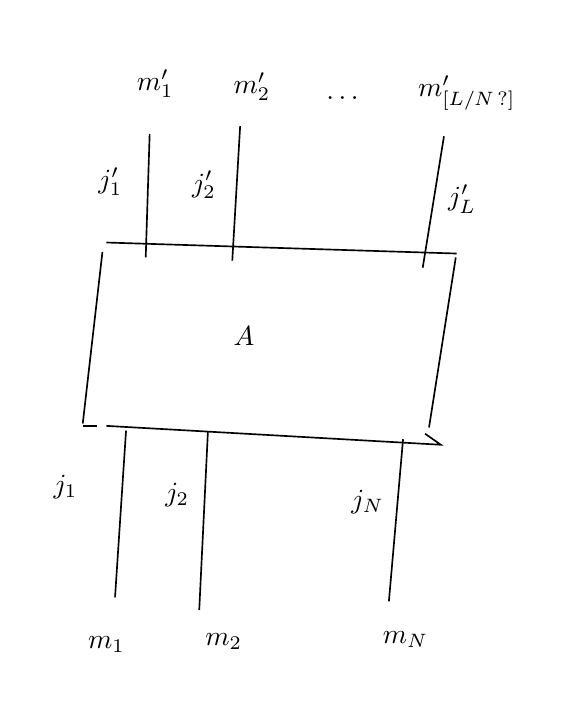
\begin{tikzpicture}[x=0.01cm,y=-0.01cm,line width=0.6pt]
\path[use as bounding box] (0,0) rectangle (665,830);
\draw (100,273)--(545,287);\draw (544,292)--(510,508);
\draw (505,516)--(525,530)--(100,506);\draw (88,506)--(70,506);
\draw (70,503)--(95,285);
\draw (155,135)--(150,292);\draw (270,125)--(260,296);\draw (529,138)--(502,305);
\draw (125,512)--(111,724);\draw (229,514)--(218,740);\draw (477,523)--(459,729);
\node at (275,392) {$A$};
\node at (105,196) {$j'_1$};\node at (224,200) {$j'_2$};\node at (552,218) {$j'_L$};
\node at (162,71) {$m'_1$};\node at (285,75) {$m'_2$};\node at (400,90) {$\ldots$};
\node at (558,83) {$m'_{[L/N\,?]}$};
\node at (48,584) {$j_1$};\node at (190,594) {$j_2$};\node at (432,603) {$j_N$};
\node at (100,784) {$m_1$};\node at (249,780) {$m_2$};\node at (480,778) {$m_N$};
\end{tikzpicture}
}
\par\smallskip{\footnotesize Частичное воссоздание видимых штрихов; неясные соединения и подписи отмечены.\par}
\end{minipage}\par\medskip


